\section{Le Kinect}

\begin{frame}
\tableofcontents[currentsection, hideothersubsections]
\end{frame}

\subsection{Matériel}
\begin{frame}{Matériel}
\vbox to 1.0\textheight
{
\begin{block}{Spécifications techniques~\cite{kinect_msdn}\cite{wiki_kinect}}
  \begin{minipage}[t]{0.49\linewidth}
    \begin{itemize}
    %\item<1-> \emph{caméra couleur}\only<1->{~:
    \item \emph{caméra couleur}
    \begin{itemize}
    \item 1280x960 à 12Hz,
    \item 640x480 à 30Hz.
    \end{itemize}%}
    %\item<2-> \emph{étalage de 4 microphones},
    \item \emph{étalage de 4 microphones}
    \end{itemize}
  \end{minipage} 
  \begin{minipage}[t]{0.49\linewidth}
    \begin{itemize}
    %\item<3-> \emph{capteur de profondeur}\only<3->{~:
    \item \emph{capteur de profondeur}
    \begin{itemize}
    640x480 à 30Hz.
    \end{itemize}%}
    %\item<4-> 
    \item \emph{moteur},
    %\item<4-> 
    \item \emph{accéléromètres}.
    \end{itemize}
  \end{minipage}
\end{block}
  \begin{center}
    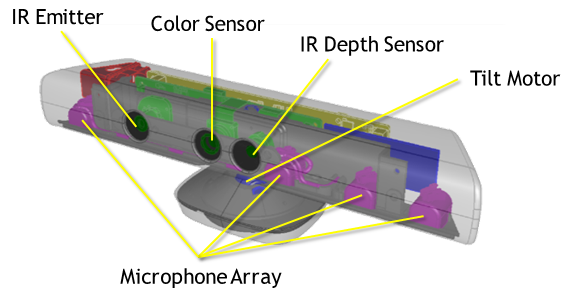
\includegraphics[height=0.4\textheight]{../images/kinect_specs}
  \end{center}
  \vfill
}
\end{frame}

%\subsection{Pilotes}
%\begin{frame}{Pilotes}

%\vbox to 1.0\textheight
%{
%  \begin{itemize}
%  \item sortie du Kinect le 4 Novembre 2010,
%  \begin{itemize}
%  \item Adafruit offre \$3000 de prime~\cite{adafruit_bounty}.
  
%  \only<1>
%  {
%  \vfill
%  \begin{center}
%  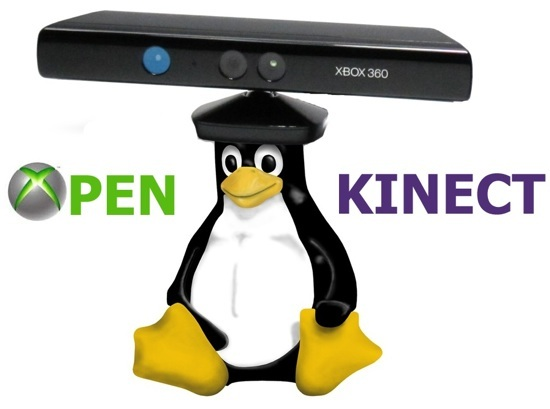
\includegraphics[width=0.65\textheight]{../images/kinect_tux}
%  \end{center}
%  }
  
%  \end{itemize}
%    \item<2-> \textbf{Libfreenect} sort le 10 Novembre 2010~\cite{adafruit_winner},
    
%    \only<2>
%    {
%    \vfill
%    \begin{center}
%    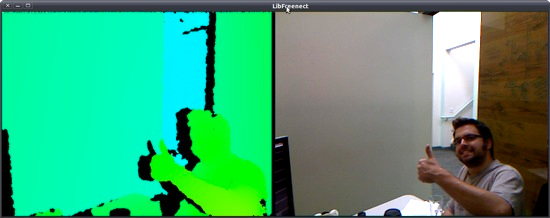
\includegraphics[width=0.9\linewidth]{../images/hector}
%    \end{center}
%    }
    
%    \item<3-> \textbf{CL-NUI} sort le 19 Novembre 2010~\cite{clnui},
    
%    \only<3>
%    {
%    \vfill
%    \begin{center}
%    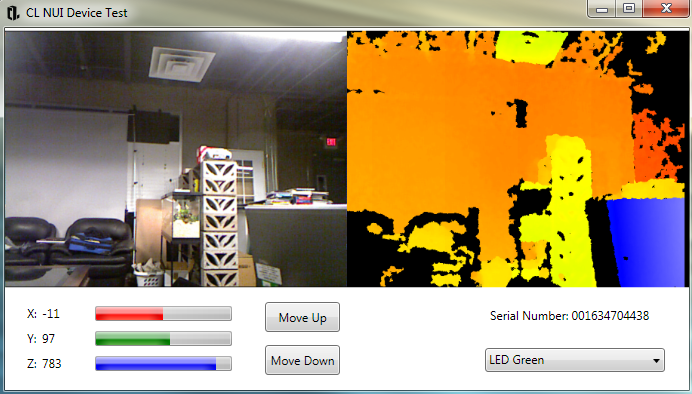
\includegraphics[width=0.6\linewidth]{../images/clnui}
%    \end{center}
%    }
    
%    \item<4-> \textbf{Kinect for Windows}~:
%    \only<4->
%  {
%    \begin{itemize}
%      \item en bêta le 16 Mai 2011,
%      \item version complète le 1 Février 2012,
%    \end{itemize}
%  }
%  \item<5-> \textbf{OpenNI SDK}.
  
%  \only<5>
%  {
%  \begin{minipage}{0.49\linewidth}
%    \centering
%    
\includegraphics[width=0.9\linewidth]{../images/openni_logo}
%  \end{minipage}
%  \begin{minipage}{0.49\linewidth}
%    \centering
%    
\includegraphics[width=0.9\linewidth]{../images/primesense_logo}
%  \end{minipage}
%  }
  
%  \end{itemize}
%\vfill
%}
%\end{frame}

\subsection{Pilotes}
\begin{frame}{Pilotes}
\begin{center}
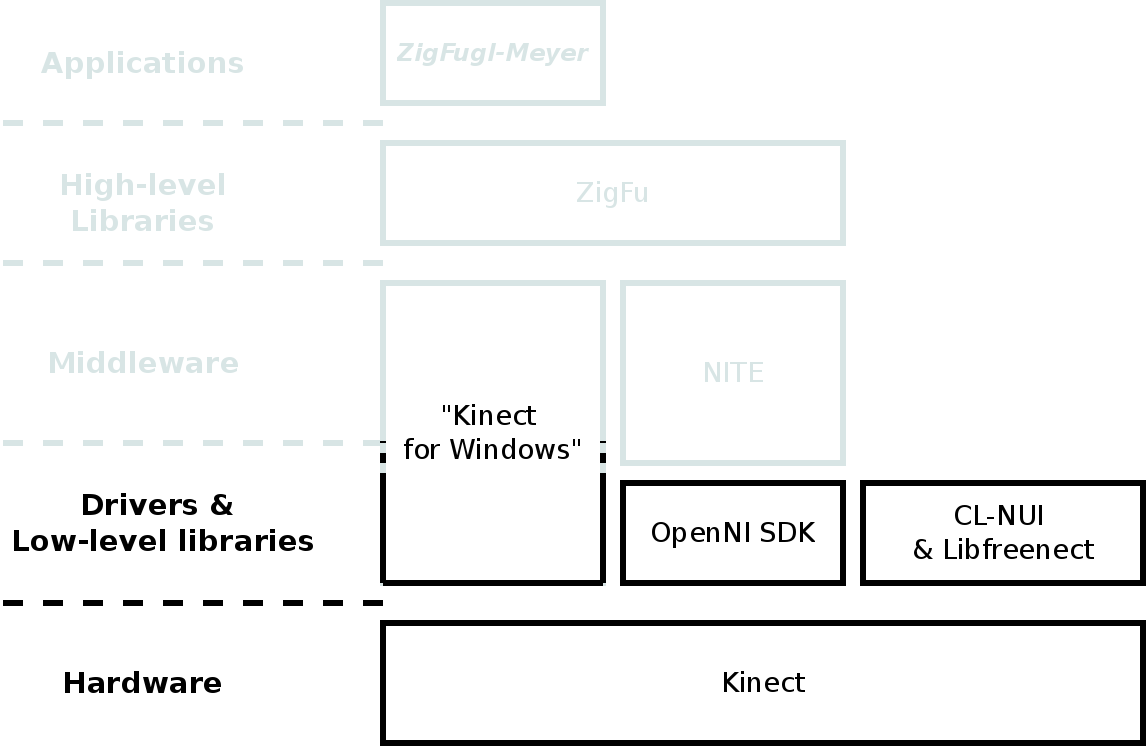
\includegraphics[width=0.9\linewidth]{../images/technology_overview_1}
\end{center}
\end{frame}

\subsection{Middleware}
\begin{frame}{Middleware}
\begin{center}
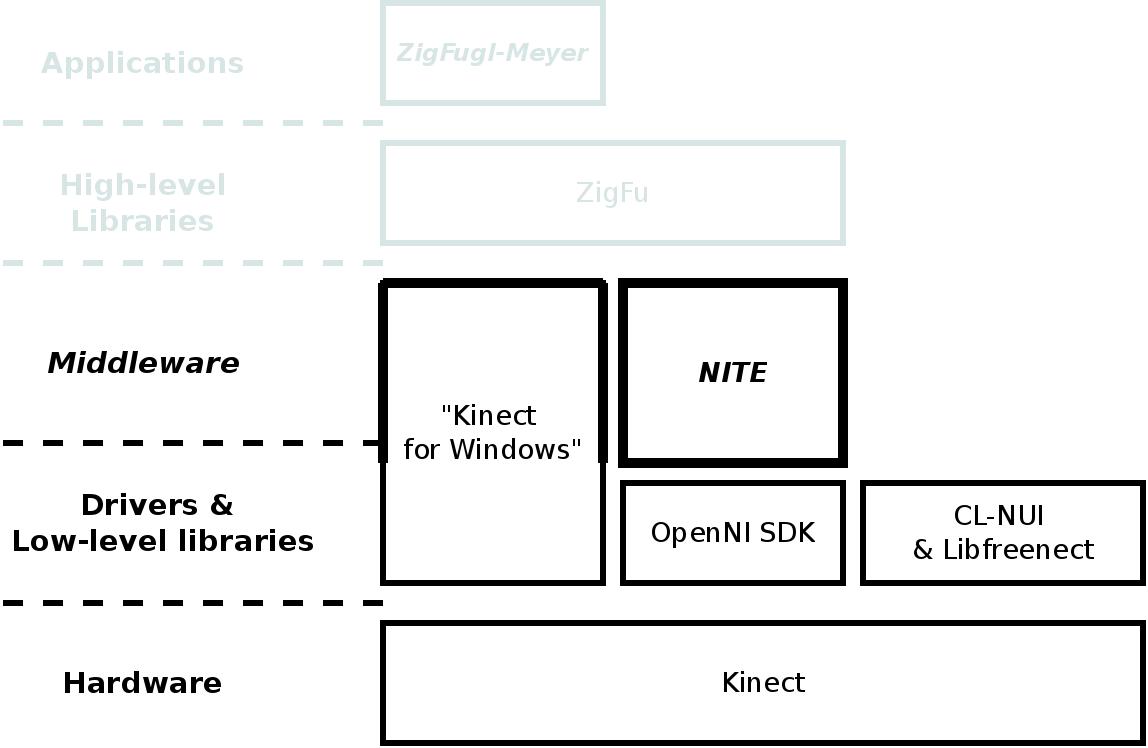
\includegraphics[width=0.9\linewidth]{../images/technology_overview_2}
\end{center}
\end{frame}

\begin{frame}{Kinect for Windows~\cite{microsoft_vs_openni_2}}
\vbox to 1.0\textheight
{
\begin{itemize}
  \item<1-> Prédictif, gère mieux l'occlusion partielle (apprentissage)
                ~\cite{how_you_become_the_controller}~\cite{shotton2011},
  \only<1>
  {
    \vfill
    \begin{center}
    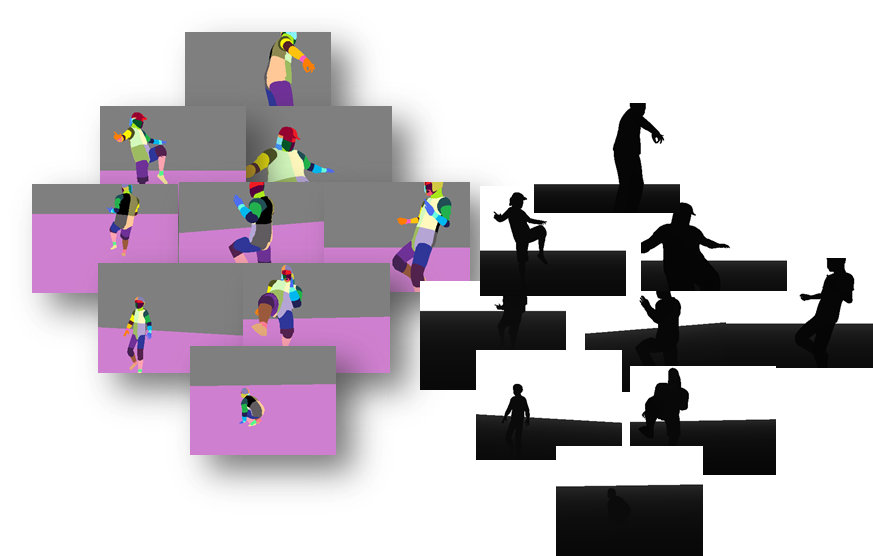
\includegraphics[width=0.7\linewidth]{../images/kinect_learning}
    \end{center}
  }
  \item<2-> Détection et suivi faciale,
  \only<2>
  {
    \vfill
    \begin{center}
    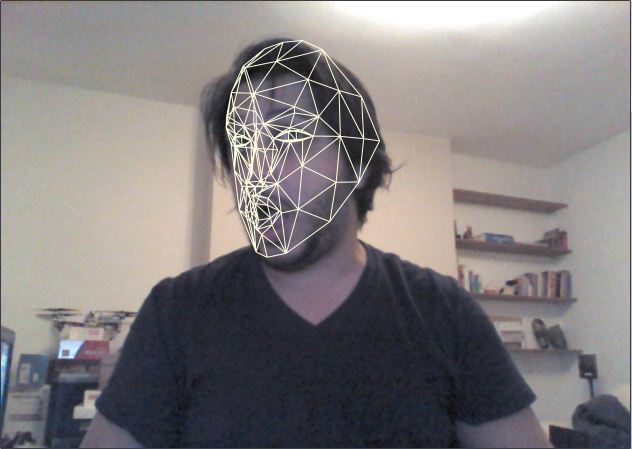
\includegraphics[width=0.5\linewidth]{../images/kinect_face_track}
    \end{center}
  }
  \item<3-> ``Kinect Fusion" ~\cite{newcombe2011}~\cite{izadi2011} et ``Interactions" depuis Mars 2013,
  \only<3>
  {
    \vfill
    \begin{center}
    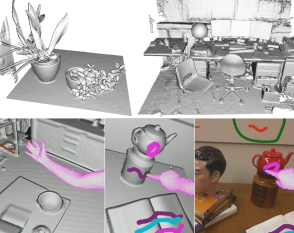
\includegraphics[width=0.4\linewidth]{../images/kinect_fusion}
    \end{center}
  }

\end{itemize}
\vfill
}
\end{frame}

\begin{frame}{OpenNI et NITE~\cite{microsoft_vs_openni}}
\vbox to 1.0\textheight
{
  \emph{OpenNI}
  \begin{itemize}
    \item<1-> Multiplateforme (Linux, Mac OS X),
    \item<2-> Standard ouvert~: middlewares alternatifs tiers,
    \only<2>
    {
      \vfill
      \begin{center}
      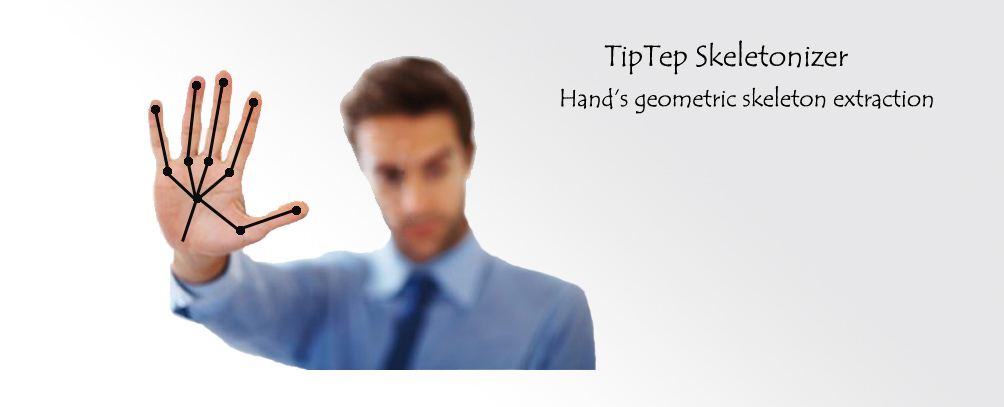
\includegraphics[width=0.8\linewidth]{../images/tiptep}
      \end{center}
    }
  \end{itemize}
  
  \only<3->
  {
  \emph{NITE}
  \begin{itemize}
    \item<3-> Moins de resources consommées,
    \item<4-> Moins de faux positives,
    \item<5-> Détection de gestes.
  \end{itemize}
  }
\vfill
}
\end{frame}

\subsection{High-level libraries}
\begin{frame}{High-level libraries}
\begin{center}
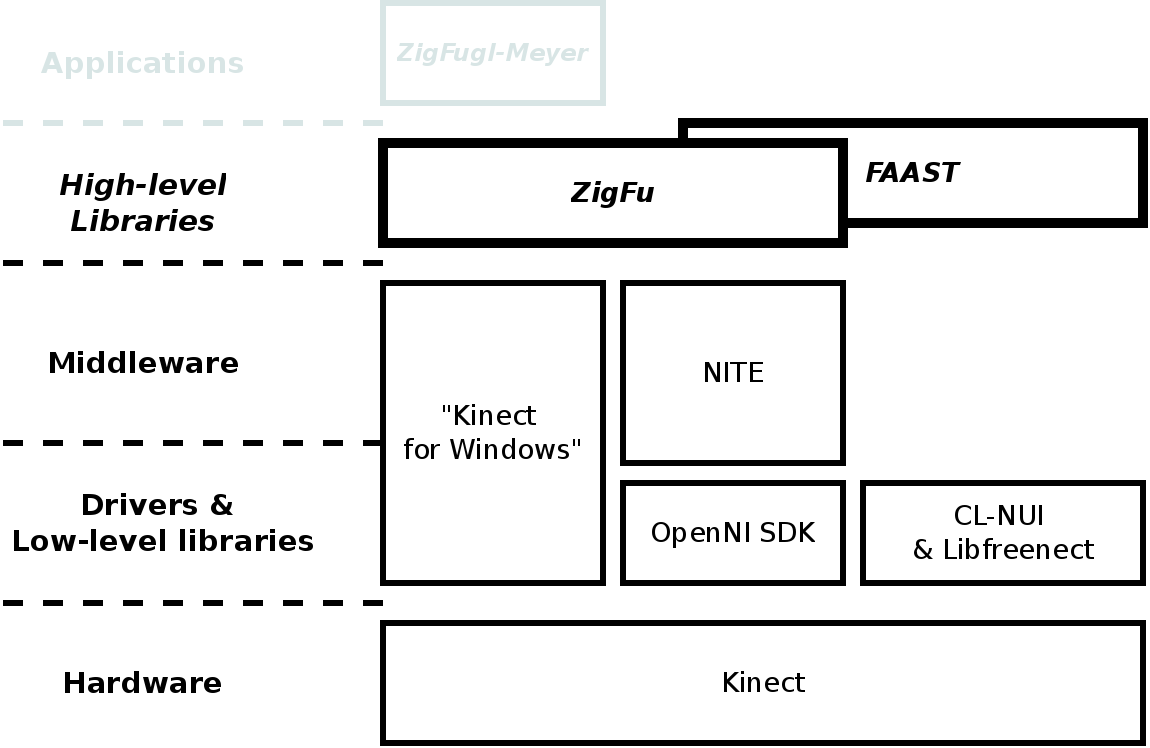
\includegraphics[width=0.9\linewidth]{../images/technology_overview_3}
\end{center}
\end{frame}

\subsection{Zigfu}
\begin{frame}{Zigfu}
\begin{block}{Features~\cite{zigfu_video}}
  \begin{itemize}
  \item Installation facile, 
  \item Bindings HTML 5, Unity 3D (et Flash bientôt),
  \item Lissage prédictif ($30 \rightarrow 60Hz$), 
  \item Cinématique inverse (simulation physique),
  \item Éléments GUI (boutons, listes, curseurs).
  \end{itemize}
\end{block}
\begin{center}

\includegraphics[width=0.2\linewidth]{../images/zigfu_logo}
\end{center}
\end{frame}

\subsection{Résumé}
\begin{frame}{Résumé}
\begin{center}
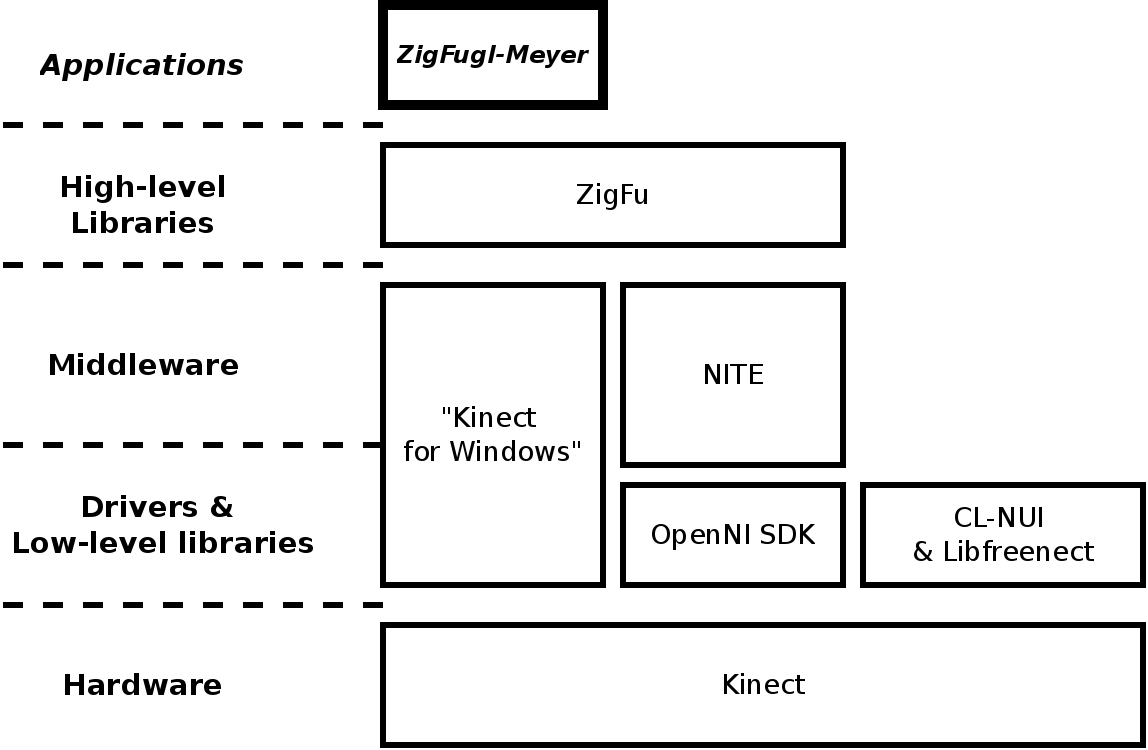
\includegraphics[width=0.9\linewidth]{../images/technology_overview_4}
\end{center}
\end{frame}